\section{Application One: Image Tracking}\label{sec:image-tracking}
Image tracking is a common application for a Bayes filter. A certain aspect of, or
object in an image is to be tracked, and the goal is to use a state
model as well as sensor measurements, to estimate its state. In the case of image
tracking the observations are usually generated by some sort of image processing
operation that identifies objects in an image. The noise inherent in these measurements
comes from the imperfect nature of this processing, i.e., we may pick up other
objects beside what we are tracking and identify these as our object.

Two example video sequences were chosen to implement object tracking. Both consist
of a single object (a ball) falling past a uniform background, hitting the ground
and bouncing a certain number of times before falling out of view.
Video sequences of this form are the easiest to track because:
\begin{compactitem}
\item The object (ball) is visible (unobscured) for the entire duration.
\item There is only a single moving object.
\item There are a number of frames at the start of the sequence in which the
ball is not visible.
\end{compactitem}
The last point is important as it allows an accurate representation of the background
to be stored by averaging the first $n$ frames in which the object is not present.
The measurements are then obtained by subtracting the background from this image.

\subsection{Observations}
The Bayes filter estimates state using (noisy) sensor measurements. In our example,
the ``sensor" is an image processing routine that attempts to identify the ball.
No feedback is used in this operation so the sensor may end up simply identifying
the largest, or most circular objects in some cases. Detection errors like these
are what make up measurement noise.

The observation algorithm used to detect the ball in each frame is shown in
pseudo-code in Listing \ref{lst:obs}.

\begin{lstlisting}[language=Matlab, label=lst:obs,
caption=Implementation of observation routine.]
% Subtract background from frame
frame = frame - background;

% Background pixels = 0, Object pixels = 1
for pixel in frame:
    if pixel != 0 then pixel = 1;

% Clean up the shape of all objects.
frame = erode(frame);

our_object = largest_object(frame)

if object is None then exit

return object
\end{lstlisting}

The measurement routine is in essence a background-subtraction, followed by some
inbuilt Matlab functions for identifying similar regions\footnote{Specifically,
\texttt{bwmorph()}, \texttt{bwlabel()} and \texttt{regionprops()}}. The result of a
typical measurement for a particular frame is shown in Figure \ref{fig:observation}.

\begin{figure}[h]
\centering
\subfloat[Original frame]{
    \label{fig:untouched}
    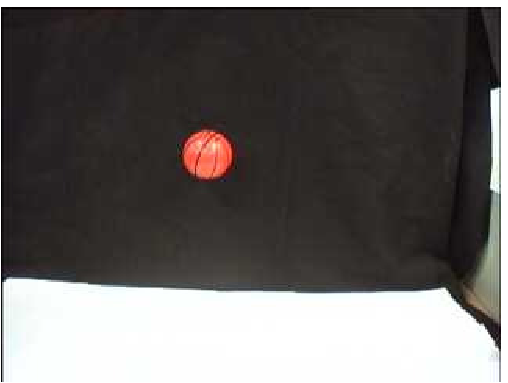
\includegraphics[width=0.4\textwidth]{images/observation/untouched}
}
\subfloat[Background subtracted]{
    \label{fig:subtracted}
    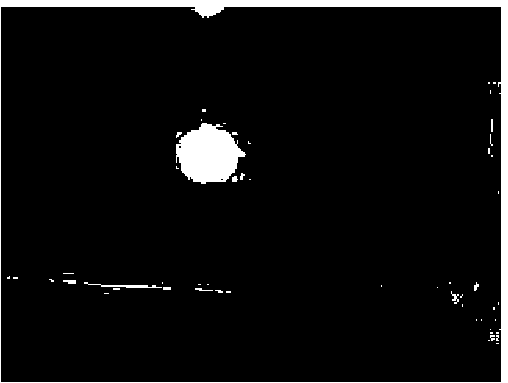
\includegraphics[width=0.4\textwidth]{images/observation/subtracted}
} \\
\subfloat[Cleaned and marked]{
    \label{fig:marked}
    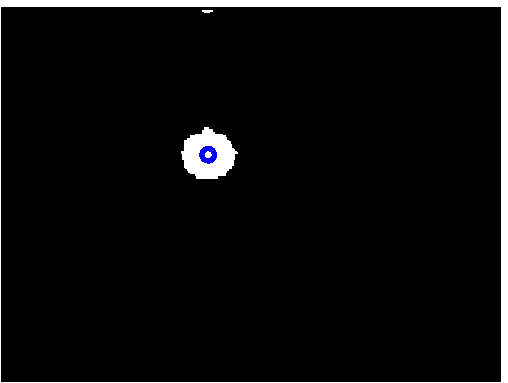
\includegraphics[width=0.4\textwidth]{images/observation/marked}
}
\subfloat[Ball successfully identified]{
    \label{fig:identified}
    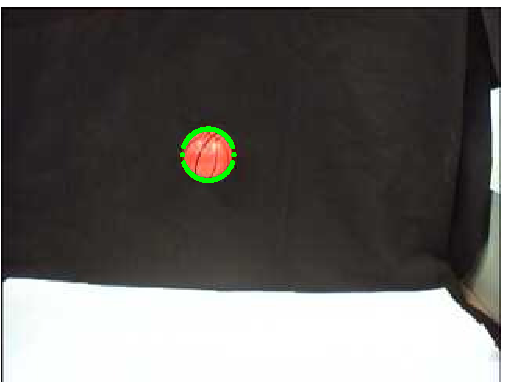
\includegraphics[width=0.4\textwidth]{images/observation/identified}
}
\caption{Sensor observation for a single frame.}
\label{fig:observation}
\end{figure}

Figure \ref{fig:untouched} shows the original frame. The ball's motion is in
a downward direction. Since we have already found the background for all frames,
we can perform a subtraction to obtain the modified frame shown in Figure
\ref{fig:subtracted}. Note that after the background subtraction a simple
routine was used to convert the image to black and white.
It is then cleaned up using inbuilt Matlab image processing
functions, and this same family of functions is also used to identify the contiguous
pixels which form the ball. As a result of the eroded image's maintaining
a circular geometry, we simply measure the ball's centre as the centre of the
white area. Were the frame to be noisier, we may lose the circular outline and
the measured centre may drift to a more incorrect value.

For illustration, the outline of the ball as measured is shown in Figure
\ref{fig:identified}. What appears to be a continuous green line is in fact
a series of green points equidistant from the measured centre using a radial
value returned from Matlab. Note again that even though the outline appears
very accurate in the chosen frame, it is possible for it to be slightly, or
completely off from the ball depending on the noise present in the image.

It is worth pointing out at this stage that such an accurate sensor eliminates
the need for a Bayes filter, as one can simply track the very accurate sensor
measurements. However, only a small amount of additional noise, or the ball's
being obstructed for several frames, would quickly necessitate a Bayes filter.
To be able to implement and test Bayesian estimation, an additional ability was
built into the measurement function to intentionally inject noise. 

The entire measurement routine was implemented as a Matlab function which
returned the coordinates (pixel locations) of the measured centre of the ball
in a given frame. This value is then used by the state space model of the system.

\subsection{State Space Model}
State space models, while important, are often extremely difficult to formulate
for real systems. However, because of the accurate sensor measurements we can
get away with an overly simplistic model, at least initially. The state space
that was chosen is shown in Equation (\ref{eq:basket-state-space}). It consists
of the 2D position of the centre of the ball and the velocity in each direction.

\begin{equation}\label{eq:basket-state-space}
\mathbf{x} =
\begin{bmatrix}
x \\ y \\ \dot{x} \\ \dot{y}
\end{bmatrix}
\end{equation}

Where $x$ and $y$ are the x- and y-coordinates respectively, and the velocity
in each direction is represented by their derivatives $\dot{x}$ and $\dot{y}$.
The positional units are with respect the the size of the image, and the velocities
in pixels per second. Having higher-order aspects of the system such acceleration
in the state space serve little purpose in this example.

\subsubsection{State Update Equation}
The simplest non-trivial model that can be applied to this system is to model
the affect of gravity. Having a dynamical model which \emph{only} takes gravity
into account will of course, break down very quickly and is not realistic. However,
it serves as a simple test.

At each time step, the positions are updated as shown below,

\begin{align}
x_{t+1} = x_{t} + \dot{x}_{t} \\
y_{t+1} = y_{t} + \dot{y}_{t}
\end{align}

That is, at each time step the positions increment by the current velocities.
The velocities are themselves updated according\footnote{The reader may notice a
perceived discrepancy in the units
at this point. It was stated that velocities are in pixels/sec, but the time
steps occur much faster than this. This is precisely the reason for the
modifications to the state matrices in Section \ref{sec:discrete}.
}
to,

\begin{align}
\dot{x}_{t+1} = 0 \\
\dot{y}_{t+1} = \dot{y}_{t} + g
\end{align}

That is, the velocity in the y-direction is incremented by the value of gravity
we choose and the velocity in the x direction remains unchanged.
It is important to keep in mind that this is simply a model we are building to
represent the behaviour of the
system; even though there is almost certainly some sideways movement of the ball,
it is probably suffice to model it as zero.

Using these equations we can begin to generate the state-space model for this
example.

\begin{align}
\mathbf{x_{t+1}} &=
\begin{bmatrix}
x_{t+1} \\ y_{t+1} \\ \dot{x}_{t+1} \\ \dot{y}_{t+1}
\end{bmatrix}
\\
&=
\begin{bmatrix}
x_{t} + \dot{x}_{t} \\ y_{t} + \dot{y}_{t} \\ 0 \\ g
\end{bmatrix}
\\
&=
\begin{bmatrix}
1 & 0 & 1 & 0 \\ 0 & 1 & 0 & 1 \\ 0 & 0 & 1 & 0 \\ 0 & 0 & 0 & 1
\end{bmatrix}
\mathbf{x}_{t} + 
\begin{bmatrix}
0 \\ 0 \\ 0 \\ 1
\end{bmatrix}
g
\\
&=
\mathbf{Ax}_{t} + \mathbf{Bu}_{t}
\end{align}
% TODO check this, its magic
Where (28) is the usual state-space form.

\subsection{Filtering Steps and Noise}
The Kalman filter implementation of the Bayes filter was used for testing. Under
the conditions of the example, that is, a linear model and linear noise,
the Kalman and particle filter methods are expected to perform identically. As
stated in Section \ref{sec:updating-bayes}, the Bayes filter has two distinct steps:
prediction and update. The implementation of the two steps differs
for the Kalman and particle filter implementations, but are described generally
below.

In the prediction step we use our simple state
model to predict the state of the system in the next time step. Since we are using
such a simplistic model, where the ball simply falls under a form of
``pixel gravity", the predict
step is not difficult to understand. It simply says that the ball will have moved downward by
$g$ pixels at each time step. This model performs well when the ball does in fact
have a downward velocity, but as expected, breaks down when the ball hits the floor
or has an upward velocity.

The update step is where we use the latest sensor measurement to correct our
prediction. It incorporates the predicted state model and the observation. Naturally,
if these values were identical (as they are when the ball is falling)
then there is no change in the update step.

In both of the two steps the noise was assumed to be Gaussian. During testing,
we simulated this noise by adding randomly distributed random numbers to both
the sensor measurements and the state update equations.

\subsection{Results}
The results for this example were not groundbreaking. The Kalman filter
implementation was first tested. As expected, the filter
tracked the object very closely while the ball had a downward trajectory, and
even when it did not, the filter still managed to stay very close. We can explain
this in terms of the (lack of) measurement noise; even when the state model broke down,
(i.e., when the ball hit the ground), the measurements were so accurate
that close tracking was still achieved.

\subsubsection{Simulated Noise}
To try and create a more realistic situation, we intentionally injected noise into
the sensor measurements and process updates. Adding additional noise to the measurement
step did not affect the tracking ability to a large extent. On the other hand,
adding only a small amount of noise to the state update step caused tracking to
become much worse. This is again entirely expected and came be easily explained
by considering our simple model. Adding noise to the update model causes two
detrimental effects, (a) the x position now changes due to noise and (b) the
effect of ``falling" under pixel gravity may now be exaggerated if a high or low
noise value is added to the model while the ball is in free-fall or rebound respectively.

Even with the added noise and the inaccurate model, close tracking was still
maintained. This can be put down to the simplicity of the actual system under
examination. A ball bouncing under gravity has only a single degree of freedom
and although the model is incorrect for half of duration of the video (while
the ball is rebounding), the measurements are still so clear that we can track
the ball accurately.

In order to prove that we were not simply following the measurements and
disregarding the state update, a final test was constructed where the measurement
noise was given an extremely high value ($\sigma = 10$) and the process noise set
to zero. When the simulation was run, tracking was started as
soon as the ball entered the frame and was maintained while the ball was
moving downward, but was lost entirely
when the ball hit the ground. This is an encouraging result and shows two things:
\begin{compactitem}
\item Recursive Bayesian estimate relies on both the state model and the observations
\item If either the measurement noise is high, or the model inaccurate, then the
other must be even more accurate to compensate.
\end{compactitem}

\subsubsection{Obstructions}
A second test of the filtering algorithm is to add an obstruction to the image.
This means that the object (ball) that we are trying to track ``disappears"
for one or more frames before coming back into view. Unfortunately, the videos
had already been taken by this stage and time did not permit a reshoot with
an obstruction added. We were able to simulate this however, by simply dropping
measurements for one or more frames.

Implementing this simulated obstruction was simple, and required only a small
change to code. As a consequence of our overly simplistic model, the
tracking was only expected to work when moving past the ``obstruction" in the
downward direction. This is indeed what was observed but it was interesting to
note just how well tracking was maintained when moving thus.
As soon as the ball disappeared, i.e., no measurement was
available, the state model of the system took over and tracked the ball down
though the obstruction. This highlights the strength of the Bayes filter, but also
the importance of an accurate model.

\subsection{Particle Filter Implementation}
Unfortunately the algorithm developed for the particle filter method did not work.
It is still not known why but we can make some assumptions about what would
have happened:
\begin{compactitem}
\item The measurements would have been identical as this was independent of the
filter implementation.
\item The tracking would have been as good or better then the Kalman implementation
due to the particle filter's ability to deal with both Gaussian and non-Gaussian
noise.
\end{compactitem}

\section{Application Two: Filtering}
We developed a second example in order to further test the properties of Bayes
filters. The image tracking example, while realistic, did not allow control of
the system, as it was simply a collection of frames that could not be changed.
Our second example involved developing a system that we completely specify, i.e.,
we have exact knowledge of its dynamical model because we created it.

The system used in the example is the spring-mass-damper described in Section
\ref{sec:state-space}. The state space derivation is already given. We can now
analyse this system in a way we could not with the image tracking example. The
goal of this application example can be stated thus: \emph{given a state-space model that is
very accurate (by definition it is perfectly accurate), and a random input
into this system, how much sensor noise can we tolerate before tracking is lost?}

\subsection{Noise}
Measurement noise in the system is by definition zero, as we can observe the
state without error. To simulate noise in the measurements, a normally-distributed
random number was added to the measurement at each time step. Manually adding this
error also means that we have knowledge of the noise variance (as we have
specified it).

\subsection{Results}
The Bayes filter was implemented as a Kalman filter because of the difficulties
obtaining results using the particle filter implementation.

Figure \ref{fig:filter} shows the results of the Bayes filter with extremely
high measurement noise ($\sigma = 10$). The true state is shown in Figure
\ref{fig:true-state}. It is a damped system starting at position $p = 10$ with
an additional random input, which is \emph{unknown to the sensor}. Figure \ref{fig:measured-state}
shows the measured state. Because of the amount of noise it is almost impossible
to make out the original signal\footnote{This is typical of signals obtained
from research into diabetes patients in which the blood-glucose level is to be
tracked.}. Finally,
Figure \ref{fig:estimated-state} shows the output of the Bayes filter.

\begin{figure}[h]
\centering
\subfloat[True state]{
    \label{fig:true-state}
    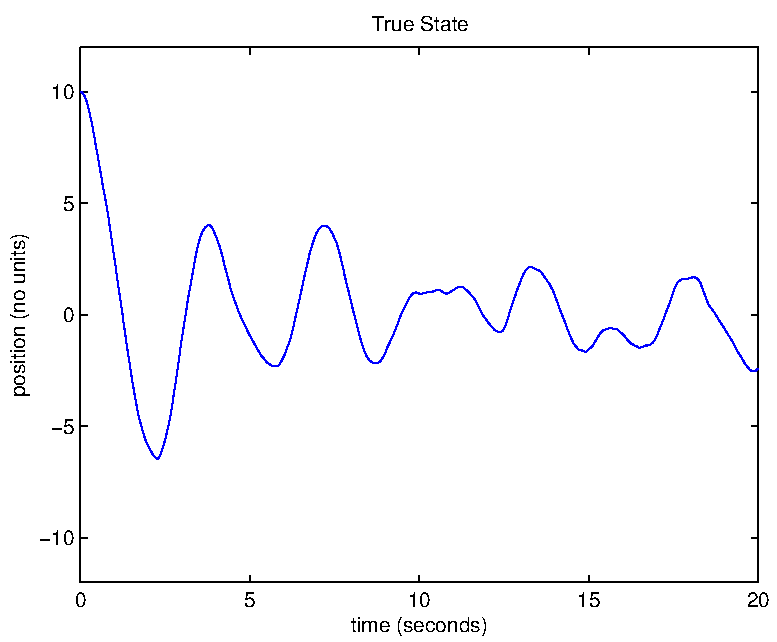
\includegraphics[width=0.4\textwidth]{images/true-state}
}
\subfloat[Measured state]{
    \label{fig:measured-state}
    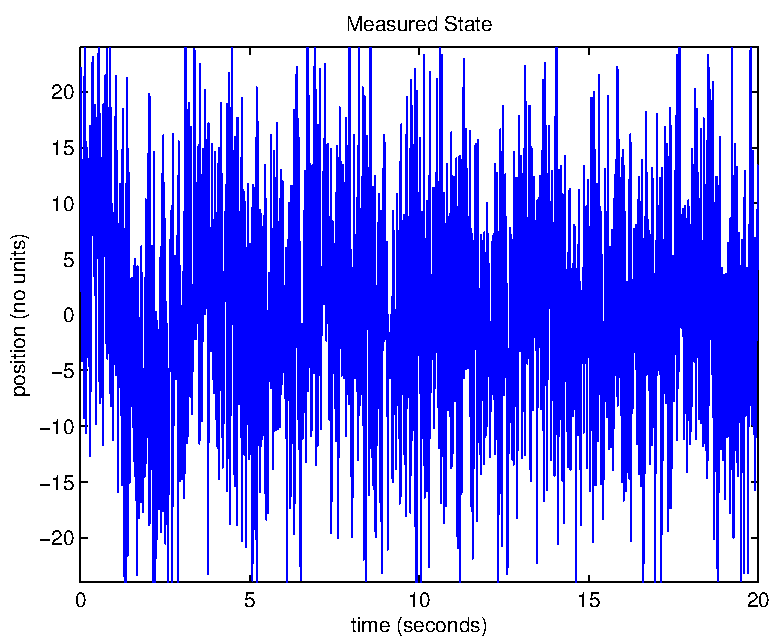
\includegraphics[width=0.4\textwidth]{images/measured-state}
} \\
\subfloat[Estimated state]{
    \label{fig:estimated-state}
    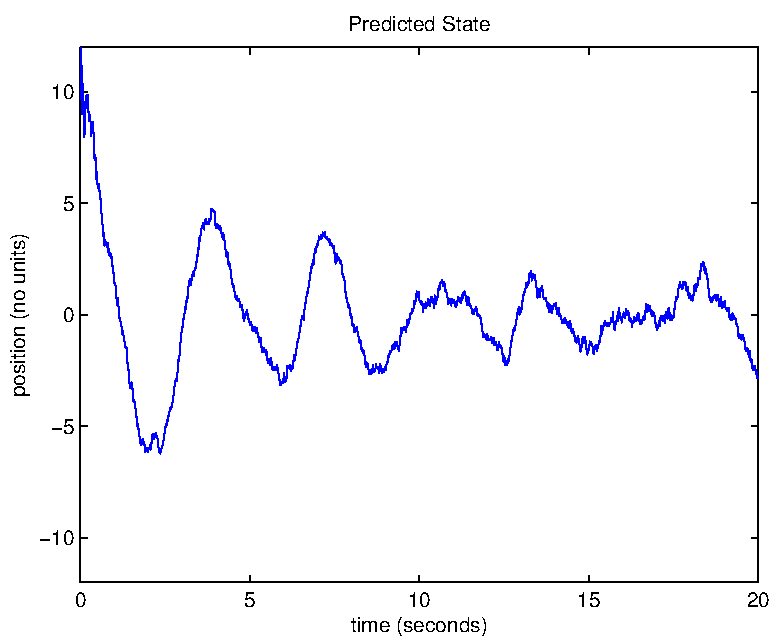
\includegraphics[width=0.4\textwidth]{images/estimated-state}
}
\caption{Tracking true state from extremely noisy ($\sigma = 10$)
sensor measurements.}
\label{fig:filter}
\end{figure}

The output maintains remarkably close tracking of the input, or stated in a
way more fitting for the example: the noise has been almost completely filtered
from the measured signal. As remarkable as this example be, it is contrived and
it is important to note the following:
\begin{compactitem}
\item Measurement noise is randomly distributed and we are aware of this fact.
\item We know the measurement noise variance \emph{exactly}.
\item We know the process noise variance \emph{exactly}.
\end{compactitem}
If either of these change, then tracking is expected to become less accurate, or
at worst, lost completely. To test this hypothesis, the true noise variance was
changed to ($\sigma = 5$) while our belief of the variance was set at
($\sigma = 2$), i.e., the sensors were poorer than the Bayes filter assumes.
The result is shown in Figure \ref{fig:filter-bad}. It is
visually obvious that the state is not being tracked accurately. This highlights
the importance of characterising the sensors so that the noise variance is
known.

\begin{figure}[h]
\centering
\subfloat[True state]{
    \label{fig:untouched}
    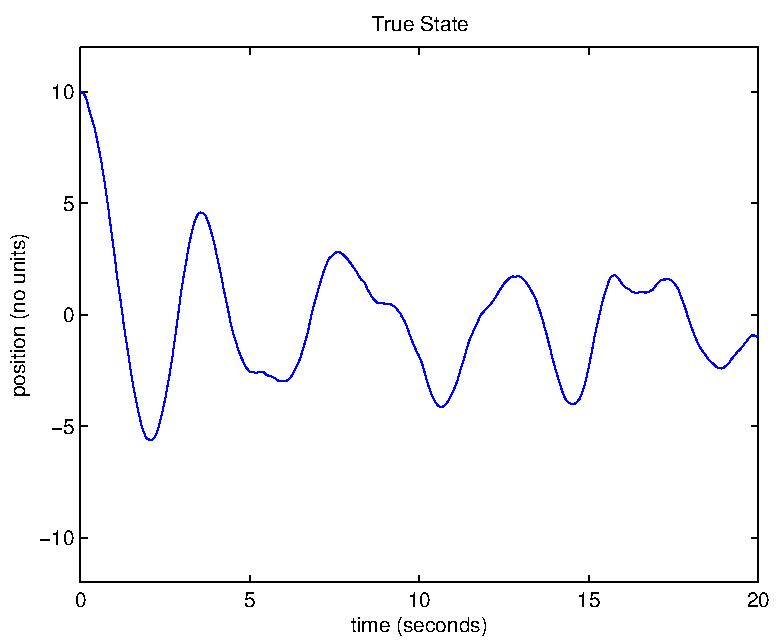
\includegraphics[width=0.4\textwidth]{images/true-state-bad}
}
\subfloat[Estimated state]{
    \label{fig:subtracted}
    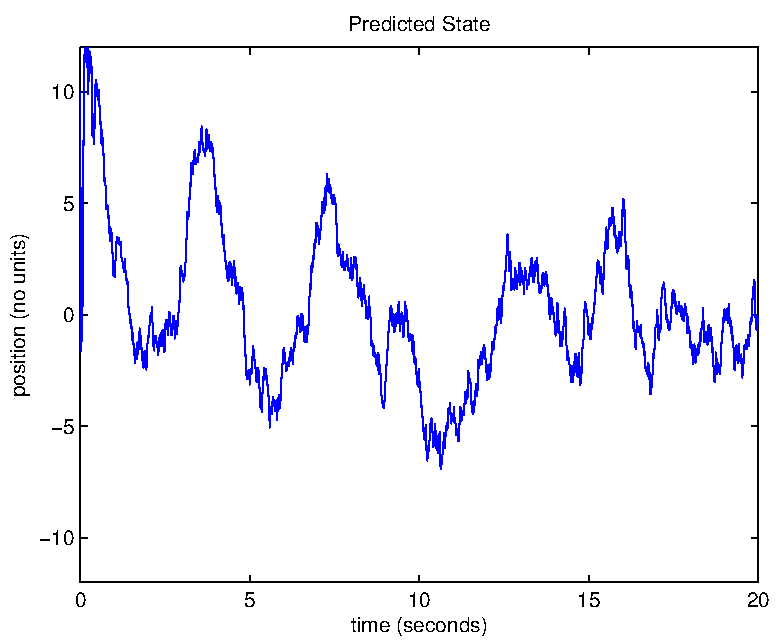
\includegraphics[width=0.4\textwidth]{images/estimated-state-bad}
}
\caption{Output when we have characterised the sensor noise incorrectly.}
\label{fig:filter-bad}
\end{figure}

The relative error between the true and estimated states for different values
of noise variance error is shown in Figure \ref{fig:noise-error}. As expected,
the more incorrect we are about the sensor noise variance, the worse tracking
becomes.

\begin{figure}[h]
\centering
\subfloat[Error = 0]{
    \label{fig:untouched}
    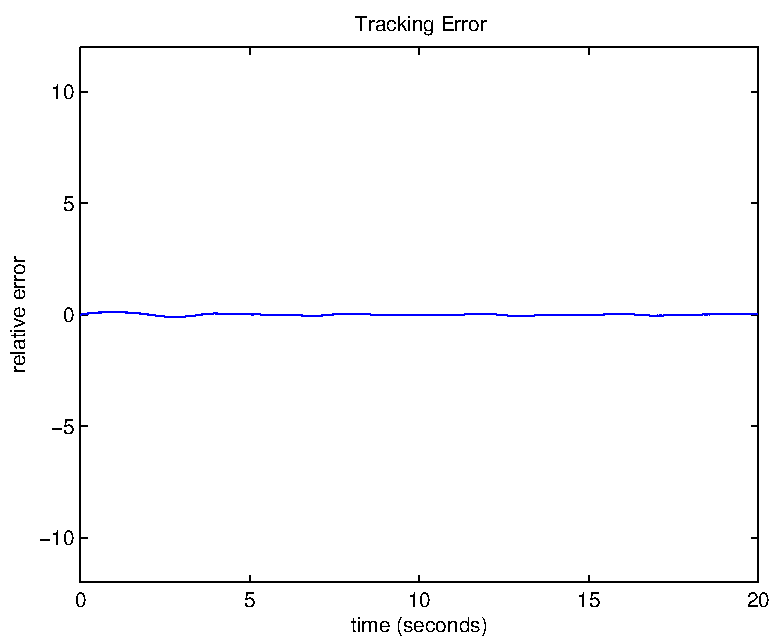
\includegraphics[width=0.3\textwidth]{images/error-state-0}
}
\subfloat[Error = 10]{
    \label{fig:subtracted}
    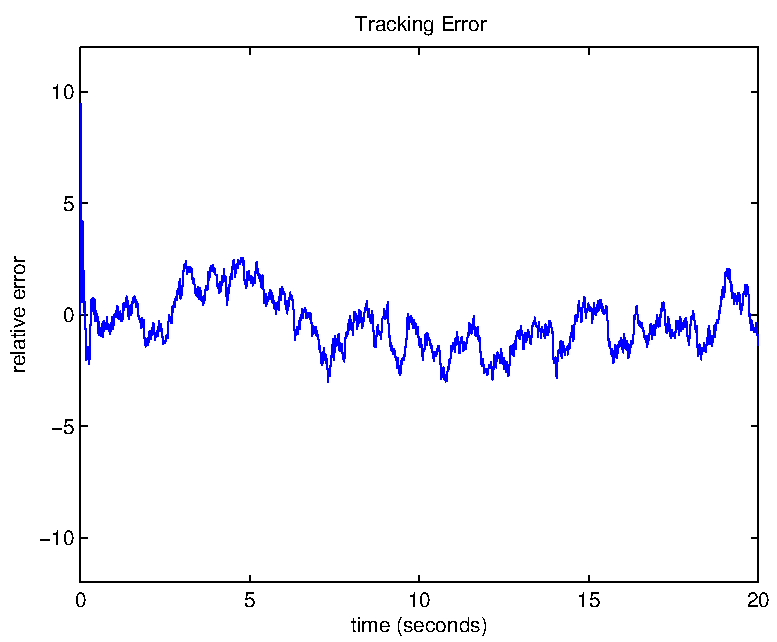
\includegraphics[width=0.3\textwidth]{images/error-state-10}
}
\subfloat[Error = 20]{
    \label{fig:marked}
    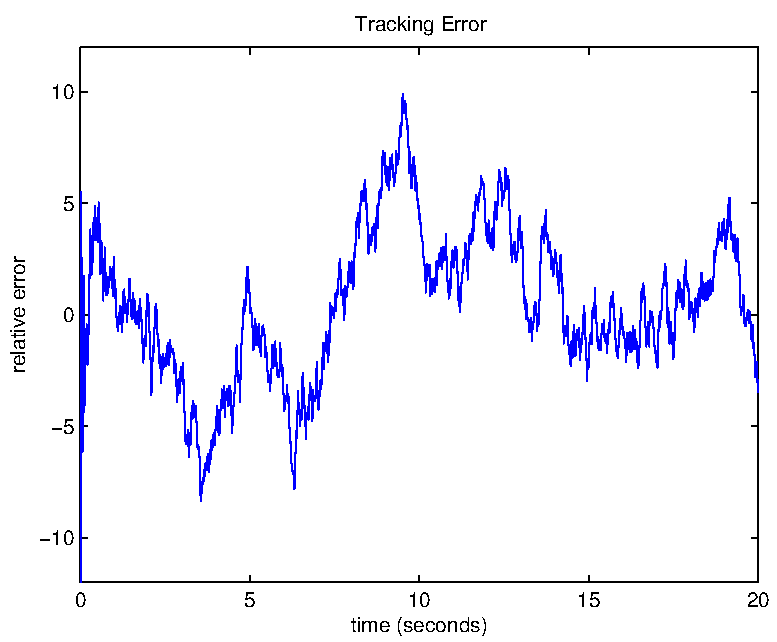
\includegraphics[width=0.3\textwidth]{images/error-state-20}
}
\caption{Changing measurement noise variance while maintaining a fixed value
of assumed measurement noise variance (unity).}
\label{fig:noise-error}
\end{figure}

\subsubsection{Particle Filter Implementation}
Even though the particle filter implementation did not work, we attempted to
create a non-linear state model, expecting the Kalman filter to fail because
of its inability to handle non-linearity in the system model.

The state model was changed to a simple non-linear system modelling a pendulum.
The derivation is omitted and only the final state-space equations are shown.

\begin{equation}
\mathbf{x}(t+1) =
\begin{pmatrix}
x_{1}(t+1) \\ x_{2}(t+1)
\end{pmatrix}
=
\mathbf{f}(t, \mathbf{x}(t)) =
\begin{pmatrix}
x_{2}(t) \\ \alpha \sin x_{1}(t) - \beta x_{2}(t)
\end{pmatrix}
\end{equation}

The same procedure was used for this new non-linear system. Unexpectedly however,
the Kalman implementation of the Bayes filter continued to work correctly.
It is unknown why this happened, but one assumption to be made is that if the
Kalman implementation functioned correctly, then the particle filter implementation
would certainly function too.

